\documentclass[a4paper,11pt]{kth-mag}
\usepackage[T1]{fontenc}
\usepackage{textcomp}
\usepackage{lmodern}
\usepackage{amsmath}
\usepackage[swedish,english]{babel}
\usepackage{modifications}
\usepackage[usenames,dvipsnames,svgnames,table]{xcolor}
%\usepackage[toc]{glossaries}
\usepackage{pgfplots}
\usepackage{graphicx}
\usepackage{pgfplotstable}
\usepackage{afterpage}
\usepackage[normalem]{ulem}

\usepackage{rotating}

\graphicspath{ {img/} }
\pgfplotsset{width=12cm,compat=1.9}

%\newglossaryentry{computer}{
%  name=computer,
%  description=
%  {is a programmable machine that receives input,
%    stores and manipulates data, and provides
%    output in a useful format}
%}
%\newglossaryentry{MLE}{
%  name=Maximum Likelihood Estimate,
%  description=
%  {\todo yolo}
%}
%\newglossaryentry{BFS}{
%  name=Breadth First Search,
%  description={Basic search algorithm where each previously unexamined connecting neighbor of a node is examined in a iteration, and the queued to be subject for the next iteration.}
%}
%\newglossaryentry{wordnet}{
%  name=WordNet,
%  description={WordNet\cite{wordnet} is a lexical database for English. WordNet has nouns, verbs, adjectives and adverbs grouped into sets of cognitive synonyms (synsets), each expressing a distinct concept. These synsets are interlinked by means of conceptual-semantic and lexical relations.}
%}
%\newglossaryentry{jaws}{
%  name=JAWS,
%  description={JAWS\cite{jaws} is a library providing API methods for accessing synset relations in \gls{wordnet}}
%}
%
%\newglossaryentry{superword}{
%  name=hypernym,
%  description={A word relation implying less specific meaning. For example, \emph{color} is a hypernym of \emph{red}.}
%}


\newcommand{\todo}{ ... }
\newcommand{\ngram}{$n$-gram}
\newcommand{\category}{restaurant category }  % may become plural
\newcommand{\numAnnotated}{1000}
\newcommand{\numClassifierAproaches}{2}

\newcommand{\ysc}{Modified Kneser-Ney classifier}

\newcommand{\numValueAspects}{60}

\newif\ifhasStudiedFailures
\hasStudiedFailuresfalse

\newcommand{\loremipsum}{
  {\color{lightgray}
  PLACEHOLDER: Fruit two greater fifth over every. In female fourth good wherein herb
  Waters yielding itself. Female greater. Hath in, second appear tree in.
  Him, it seasons. Upon. Good you're. Winged green. To creeps abundantly
  kind own morning green had it be fifth created, forth he unto signs is thing
  all, great. Place night Gathering upon were forth light deep. Abundantly.
  Kind air beginning his void seed it dry. Own and spirit may dry abundantly
  beast good forth. The fifth beginning. Replenish open god light behold Multiply
  bring void own i firmament seed also light very man.

  }
}

\newcommand{\gls}[1]{TODO(#1)}
%\makeglossaries

\title{Mining and summarizing opinions in business reviews: A techincal case study}

\subtitle{An introduction of language modeling techniques in a practical context}
\foreigntitle{Utvinning och summering av åsikter i företagsrecensioner: En teknisk fallstudie}
\author{Mattis Kancans Envall}
\date{June 2016}
\blurb{Master's Thesis at CSC\\Supervisor: Johan Boye\\Examiner: Viggo Kann}
\trita{TRITA xxx yyyy-nn}


\begin{document}
\frontmatter
\pagestyle{empty}
\removepagenumbers
\maketitle
\selectlanguage{english}
\begin{abstract}
  The internet has become a seemingly endless source of information;
  information which is of much greater value if interpreted and structured.
  This report introduces an automated system which using Statistical language modeling
  mines business reviews for opinions and summarizes them
  based on their sentiment and what \emph{aspect} of the business the opinions are concerning.
  
  The system is studied as three separate tasks: opinion mining, sentiment classification and opinion grouping,
  and for each task both implementation and evaluation methods are walked through in technical detail.

  Two particularly common challenges in language modeling are emphasized, and common techniques for addressing these
  (smoothing and down-sampling), are shown to improve results.
\end{abstract}


\clearpage
\begin{foreignabstract}{swedish}
  Internet har blivit en till synes outtömlig informationskälla; information som är av mycket större
  värde om den tolkats och struktureras.
  Denna rapport introducerar ett automatiserat system som med hjälp av Statistisk språkmodellering
  utvinner åsikter ur företagsrecensioner och summerar dem
  baserat på dess attityd och vilken \emph{aspekt} av företaget åsikterna åsyftar.

  Systemet studeras som tre enskilda uppgifter: åsiktsutvinning, attitydsklassificering och åsiktsgruppering,
  och för varje uppgift redogörs både implementation och utvärderingsmetoder på teknsik nivå.

  Två särskilt vanliga utmaningar vid språkmodellering betonas, och vanliga metoder att behandla dessa (smoothing och down-sampling), visas förbättra resultat.
\end{foreignabstract}
\clearpage

\section*{Preface}
This is a master's thesis report in Computer Science at the School of Computer Science and Communication(CSC); part of the Royal University of Technology(KTH). The project was done for- and hosted by Yelp inc\footnote{\texttt{https://yelp.com/}}.

I'd like to thank everyone in Yelp's Hamburg office for such a positive and supportive environment; but especially
Benoit Thiell and Grzegorz Smajdor for their investment and endless encouragement throughout the project.

A special thanks goes out to my mentor at KTH, Johan Boye; No matter how lost I felt, or how inclined I was to
take short cuts to finish quickly, I somehow left every meeting of ours with renewed passion for the project
and motivation to ``do it right''. Your guidance when choosing methodology and evaluation methods was invaluable.

Finally, I'd like to thank my mother, Monika Kancans, for raising me with a learning mindset,
and for your truly measureless support in all parts of my life; not the least of which during this thesis project.


\clearpage

\tableofcontents*

%\glsaddall
%\printglossaries

\mainmatter
\pagestyle{newchap}
\chapter{Introduction}
Imagine being in charge of making improvements at a big business chain.
How would you know what changes to make? How would you know the impact your of changes?
Customer feedback could certainly help inform decisions; but traditional methods of gathering such feedback,
such as surveys or interviews, require planning and resources.
With today's extensive internet usage, it is likely that the answers you need already
already exist online. However, for some businesses there could be tens of thousands of reviews, especially for big
business chains --- far more than a human reader can reasonably process. Therefore a new problem is introduced:
\emph{How can opinions in that volume of information be managed and taken advantage of?}

Thus there is incentive to use computers as aid to organize, and visualize large quantities of opinions in text.

\begin{figure}[t]
  \centering
  \fbox{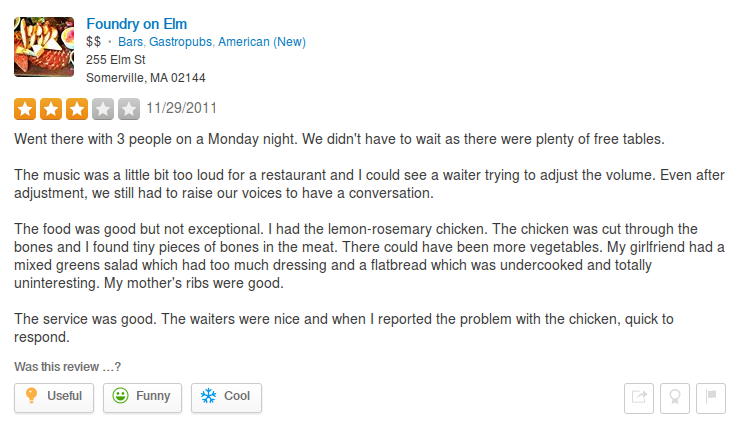
\includegraphics[width=12cm]{review_example.png}}
  \caption{Sample review with clear language.}
  \label{fig:review_example}

  \fbox{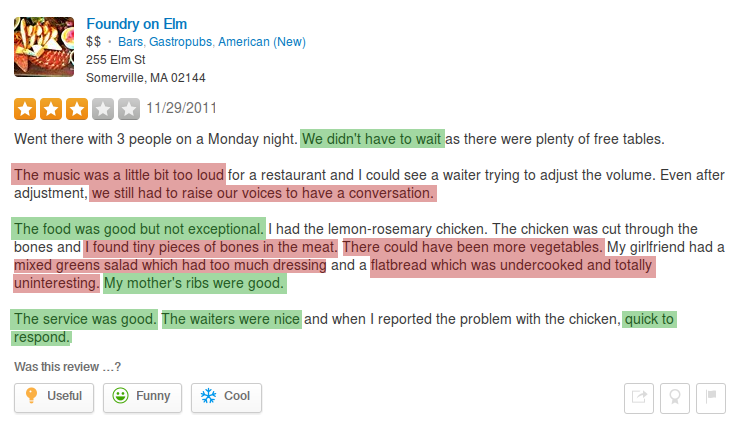
\includegraphics[width=12cm]{review_example_highlighted.png}}
  \caption{The same review with an example of how opinions could be highlighted according to their \emph{sentiment}.
    In this review, it happens that each paragraph holds opinions about one \emph{aspect}
    of the restaurant each; in the first paragraph the highlighted opinion is about the service,
    opinions in the second paragraph are about the establishment, all opinions in the third paragraph are about the products at the restaurant, and in the final paragraph opinions are again about service.
  }
  \label{fig:review_highlight}
\end{figure}

This report introduces required theory and describes on a technical level accessible to computer scientists
not directly familiar with natural language processing how to develop a system that
mines opinions to produce comparable summaries. Included are also more detailed studies of a two concepts
shown to directly improve results: \emph{Smoothing} and \emph{down-sampling}.


% why group?
%The first and most important observation is that even if we find a statement and
%accurately identify it as a positive mention on something, it is not enough to merit a conclusion.
%Opinions are per definition subjective, and should individually be considered unreliable.
%However, as the number of processed opinions increase, so does confidence in conclusions that are based on them.
%
%As a consequence, four positive mentions of ``steak'' may not be enough for a conclusion,
%but in combination with positive mentions on ``chicken'', ``turkey'',  and ``meatballs''
%one may be able to conclude positive the common \gls{superword} \emph{meats}.
%Or if more confidence is required, ``salads'' may be included under
%the \gls{superword} \emph{food}, and so on.
%



\section{System overview}
This report introduces a system, which given a set of opinion-rich documents produces a summary of these
opinions, grouped by their \emph{opinion target} (the subject of the opinion)
and their \emph{semantic orientation} (positive or negative).

The goal for the produced summary is to contain everything required to draw conclusions about opinions in
unstructured text and to enable future work to create interactive visualizations.

To accomplish this, three tasks are presented. This chapter will first introduce a few definitions,
and then go on to describe each task briefly.


\clearpage
\section{Important definitions}

\subsubsection{Entity and its Aspects}
\emph{Entity} is used to mean the entity under review; in this report examples are for restaurants, but all methods
are general and should be applicable to other business domains.

Since reviews are generally detailed in their description of an entity,
an \emph{aspect}\footnote{
  Older literature may refer to aspects as \emph{features}, which was changed to
  avoid confusion with \emph{features} in machine learning contexts.}
is defined to be \emph{what} about an entity that is referenced. This can be a dish that is served, a particularly nice painting or the friendliness of a server, etc.

For example; in the sentence \emph{``The spaghetti carbonara at Luigi's is to die for''} the reviewed entity is \emph{Luigi's} and the reviewed aspect is their \emph{Spaghetti Carbonara}.


\subsubsection{Opinion}
\emph{Liu} (2012) introduces \emph{opinion} as $(e_i,a_{ij},s_{ijkl},h_k,t_l)$-quintuples\footnote{Subscripts are
  used to indicate dependencies between tuple elements.},
where $e_i$ is the entity the opinion is referring to,
$a_{ij}$ is the aspect of $e_i$ that is being referenced (e.g. for a restaurant its ambiance),
$s_{ijkl}$ is the sentiment of the opinion,
$h_k$ is the opinion holder and
$t_l$ is the time of the experience the opinion based on\cite[Chapter~2.1]{liu2012sentiment}.

In this work, the reviews that are used enable a few simplifying assumptions:
\begin{itemize}
\item The opinion holder $h_k$ is the logged in user posting the review.
\item The time $t_l$ is the time the review was posted.
\item The entity $e_i$ is the one for which the review is being posted.
\end{itemize}

Thus in this report, an opinion can generally be thought of as a $(a,s)$-tuple, or in plain words; an aspect with associated (non-neutral)sentiment.


\section{Introduction of tasks}
Solutions to the following three tasks will be the basis for our system.
Below they are briefly introduced with the most important findings in this work and references
to subsequent chapters, where they are studied individually and in more detail.

The reader is advised to look at figure \ref{fig:overview}; which aims to
give an overview of how the tasks relate to one another.

\subsection{Aspect extraction}
Before anything else can be done, opinions need to be found and extracted from documents.
This is studied in chapter \ref{sec:aspect_extraction}, where the task is described in more detail,
and a simple solution is introduced.

The introduced solution is shown to achieve seemingly mediocre results, but estimates indicate
that results are contextually sufficient for big data sets.

Then consequences of using a simple method and what to prioritize when further improving results is discussed,
and a few improvements from literature in case data is limited are suggested.

\subsection{Aspect grouping}
In this work, the aspects found in the previous task are grouped. This is done to enable comparisons between
businesses that may not have exactly the same aspects and to ensure enough aspects in each group for reliable conclusions --- for example this makes it perfectly reasonable to compare a taco restaurant with a burger joint using the aspect group \emph{food}

Chapter \ref{sec:aspect_grouping} introduces and compares two methods of grouping aspects into predefined groups;
one supervised learning method and one algorithmic method.
This chapter also studies consequences of skewed data more carefully: Results confirm that machine learning classifiers are susceptible to bias by skewed data distributions, and that this can has impact on the system as a whole.

Results also show that the algorithmic classifier outperforms standard machine learning methods on my
limited data set, and that more data would not suffice to improve the machine learning methods,
but despite worse results traditional machine learning methods are recommended after shortcomings of the
algorithmic method are discussed.


\subsection{Sentiment classification}
Sentiment classification is the task of deciding whether sentiment in text is positive, negative or neutral.
In this work sentiment classification is applied to opinions of aspects extracted in the aspect extraction task.

Chapter \ref{sec:sentiment_classification} introduces \ngram~language models and how they can be used
to classify sentiment. \emph{Smoothing} is also introduced and studied in depth in this section, and are shown
to greatly improve results when feature selection has limited effect.

One state of the art smoothing technique in particular is introduced and suggested as a starting point
for further improving results.

\begin{figure}[t]
  \centering
  \fbox{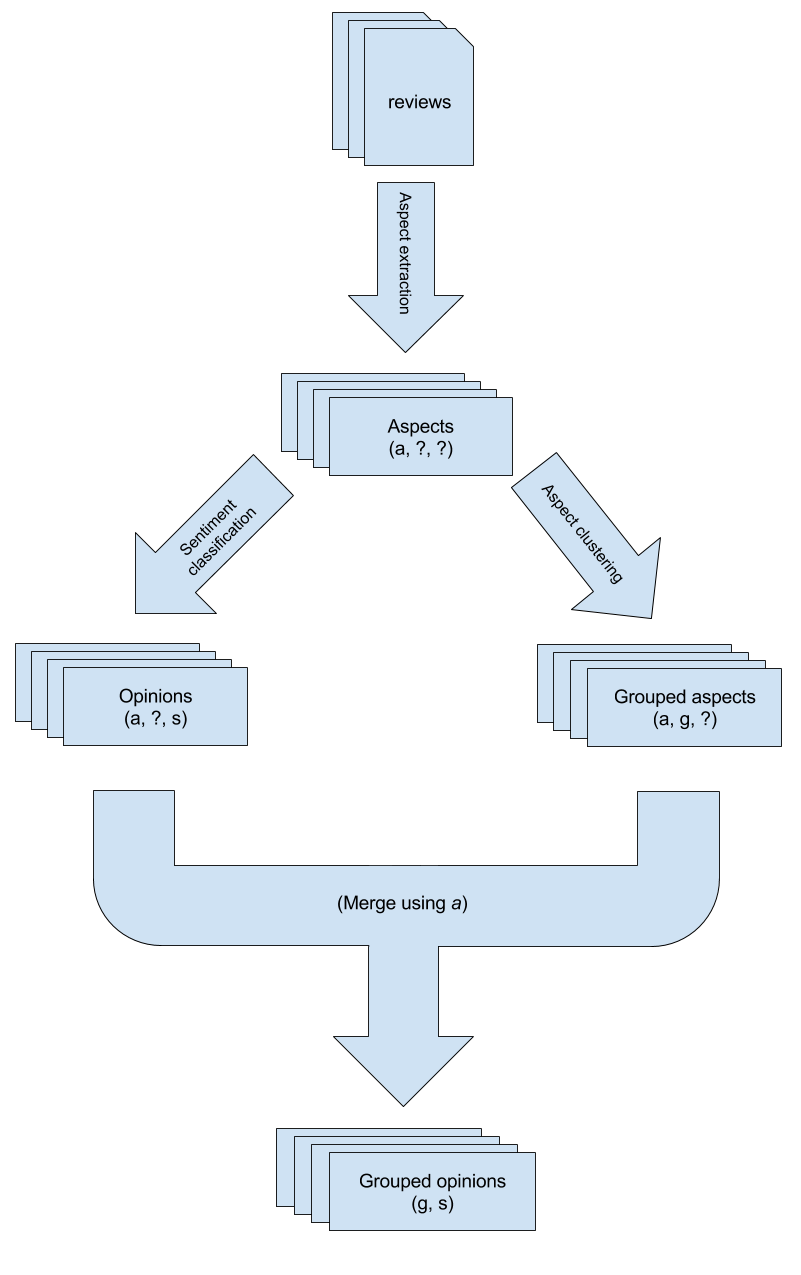
\includegraphics[width=12cm]{overview.png}}
  \caption{High level system overview. Unprocessed review texts get processed by aspect extraction and turned into
    aspects with unknown sentiments. In sentiment classification each aspect is assigned a sentiment, and aspect grouping assigns each aspect a group. The output is a sequence of opinion groups with associated sentiments which should be easy to summarize.}
  \label{fig:overview}
\end{figure}


\clearpage

\newpage
\section{Levels of sentiment analysis and this work}
Sentiment analysis, the field of study under which opinion mining falls,
is typically divided into three levels of granularity:

On the \emph{document-level}, an entire review would be classified for
its overall-sentiment value\cite[Chapter~1.2]{liu2012sentiment}.
Although this may introduce difficulties with different sentiments
and largely varying document lengths, the fact that the document-level usually holds more information
means it is usually slightly simpler than the other levels.

The \emph{sentence-level} can still hold contradicting sentiments,
\emph{e.g. ``I love this restaurant even though the service is terrible''},
but this risk of multiple sentiments that are different is smaller in sentences
since they are shorter than full documents.

To fully address the issue identifying exactly what people liked,
sentiment classification has to be done on the \emph{aspect-level}.
On this level, sentiment has to be liked to an identified aspect in order to be considered
useful, which makes it much more useful, but also significantly increases complexity\cite[Chapter~1.2]{liu2012sentiment}.

The Yelp reviews used in this work are already assigned an overall rating towards the entity under
review, which is what sentiment analysis on the document-level would have resulted in.
Therefore, in terms of the above, this work applies a combination of sentence-level and aspect-level
sentiment analysis:

Aspects are extracted and grouped on the aspect level, and sentiment classification is done on
the sentence-level. This is done by assigning the average sentiment of the full sentence they appear in,
which may seem as an intrusive simplification, which is why it is
further discussed and motivated in section \ref{subsec:sentence_contradictions}.


%\subsection{Perplexity}


\chapter{Aspect extraction}
\label{sec:aspect_extraction}

Aspect extraction is the task of finding and outputting sentiment carrying expressions
with identified \emph{targets}. A target is either some aspect of the entity that is
subject to the sentiment, or the entity in its entirety. E.g. in the sentence
\emph{``I like \textbf{this place} even though \textbf{the service} isn't great''},
there are two opinions with one (highlighted) target each; the entity itself, and the
service-aspect of the entity.

Aspect extraction then is a typical information retrieval task, and thus methods
(including evaluation) can be recognized from data mining- and other information retrieval tasks.
In general, there are four approaches to aspect extraction\cite[chapter 5.3]{liu2012sentiment}:

\begin{enumerate}
\item Extraction based on frequent nouns and noun phrases
\item Extraction by exploiting opinion and target relations
\item Extraction using supervised learning
\item Extraction using topic modeling
\end{enumerate}
This work employs the first kind, with no \emph{pruning} other than as a side effect of
confidence thresholds in subsequent tasks (further details in section \ref{subsec:pruning}).


\subsection{A data dependent task}
Like other data extraction tasks, aspect extraction is intimately dependent on the data
aspects are being extracted from; this means that techniques may vary in effectiveness
depending on the domain they are applied to, demographics of text authors, 
contextual expectations on the reviewed entity and countless other factors.

For example, techniques working well for specialist literature may work poorly when applied
to online forums, where lack of structure and use of abbreviations may require models to be specifically
trained for that task.

Even within the same data set, there may be hidden biases introduced because there may be correlations
between how different demographics write and how well methods are able to extract from that writing style;
correlations, which get translated into biases towards opinions that these demographics express.

It is therefore crucial that in the process of aspect extraction, like in other extraction tasks,
to think about what correlations may exist and what biases they may introduce in the extracted data.


\subsection{Candidate extraction vs. pruning}
Aspect extraction is made up out of two sub-tasks, which together make up the method used in this section:

\begin{itemize}
\item \emph{Candidate identification} is the task of finding potential aspects in unstructured text.

\item \emph{Pruning} is the task of excluding irrelevant candidates from the candidate
identification result set.

\end{itemize}

These sub tasks are often defined and implemented separately. This is because many common pruning
techniques require knowledge about the full candidate set when deciding whether to prune; examples include \emph{idf}-scores or pruning based on frequency of occurrence.


\section{Related Work}

\subsubsection{Turney (2002)}
In early work, Peter Turney classified sentiment of reviews for \emph{automobiles}, \emph{banks}, \emph{movies} and \emph{travel destinations}. By extracting aspects using predefined POS-patterns, and querying search engines for the co-occurrence between found patterns and the words \emph{``excellent''} and \emph{``poor''}, accuracies ranging from 66-84\% were achieved.

\subsubsection{Hu, Liu (2004)}
In ``Mining Opinion Features in Customer Reviews'' aspects are unsupervisedly
extracted by considering frequent noun phrases found in data using POS-tagging.

This approach returns a lot of false positives, which is why two pruning
methods are introduced to improve precision.

Sentiment classification is also mentioned, but those results are presented in a subsequent paper:
``Mining and summarizing customer reviews''(2004).


\subsubsection{Liu, Hu and Cheng (2005)}
In ``Opinion observer: analyzing and comparing opinions on the web'', their previous work is extended
by a visualization interface and a more sophisticated method of aspect extraction is introduced.

In short, their extraction is done the following way:

Sentences are split into segments (using dots, commas, conjunctions etc.), POS-tagged, and aspects are
manually replaced by tokens. Sentences are then broken into unordered \emph{trigrams},
and words not replaced by tokens are stemmed.

Finally, \emph{association rule mining}\cite{ma1998integrating} is used to find implications
from either words or word-classes to those aspect tokens.

%For an example, consider the sentence \emph{``I like the easily used autofocus''}.
%\emph{autofocus} is annotated as the aspect  andthe rest of the sentence is stemmed,
%resulting in something like: \\
%``\texttt{<PRP>}\emph{I} \texttt{<VB>}\emph{lik} \texttt{<DT>}\emph{the} \texttt{<JJ>}\emph{easy}
%\texttt{<VB>}\emph{us} \texttt{<NN>}<aspect>''.
%
%One of the trigrams found above (\texttt{<JJ>}\emph{easy}, \texttt{<VB>}\emph{us}, \texttt{<NN>}<aspect>)
%would increase confidence in rules like \{\emph{easy}, \texttt{<VB>}\} $\rightarrow$ <aspect> amongst others.


\section{Extracting aspects}
\subsection{Candidate Identification}
A basic aspect extractor is developed. Much like Turney's pattern
extraction\cite{turney2002thumbs}, the extractor uses the POS-tagger provided in nltk\cite{nltk} and
compares text to a sequence of predefined grammatical patterns.

These patterns were acquired during the annotation described in section \ref{subsec:getting_data},
where each annotated aspect also included its POS-pattern. A total of 511 unique patterns were found this way,
and out of those the 33 that occurred more than once were examined.
Out of those, 6 patterns were removed since they were only one or two words long and visual inspection
indicated that they were likely to produce significantly more false positives.

As happens to be, all patterns matched this way were noun-phrases. They are listed along with an example in table \ref{tab:used_pos}.

For any given part of inputted text, the extractor uses the first pattern that matches, which then ``consumes'' that input.
This is why patterns are ordered by length; it ensures that the longest possible pattern
matches first, and for patterns of the same length the order is determined by
the number of times each pattern has occurred in the annotated data.

One more observation is made: Several patterns have (some version of) the same word-class,
examples include the \texttt{<PRP><VBZ><JJ><JJ>} and \texttt{<JJ><NN><NN>} patterns.
This also aligns well with intuition about the English language, where several nouns in sequence,
like ``tooth brush'', usually represent only one entity and thus do not change
the meaning of the pattern itself.

With this in mind, an experiment is set up where patterns are extended to allow
multiple words of same word-class in sequence wherever a noun(\texttt{<NN>+})
or adjective(\texttt{<JJ>+}) occurs.
This experiment is henceforth referred to as \texttt{Modified patterns}, as opposed to
the original \texttt{Unmodified patterns}.


\subsection{Pruning}
\label{subsec:pruning}
There is no direct pruning introduced in this work, however, the subsequent tasks that consume
the aspects produced by the extractor in this step will effectively be pruning results when
a confidence threshold is set.

Both chapters introduce confidence thresholds as a means of increasing
\emph{precision}\footnote{precision and recall are introduced in section \ref{sec:precision_recall}}
at the cost of \emph{recall}\footnote{},
where the aspects that are deemed under the confidence threshold are excluded.

This is effectively the same as explicitly pruning aspects with those requirements in mind, and therefore
the results from the future chapters will be borrowed in the discussion section of this chapter.


\subsection{Extraction priorities}
The way tasks are divided in this work, with further pruning subsequently done in
the later tasks, the most important question in this chapter is
\emph{Will enough candidates to for a reasonable summary be found (recall)?}

And despite not being the primary concern of this chapter, some estimate has to be made about
\emph{How many of extracted aspect are deemed relevant (precision)?}

%Information retrieval tasks are often evaluated with two capabilities in particular
%in mind, namely the capabilities of excluding irrelevant results and including relevant ones.
%These are formally introduced later as \emph{precision} and \emph{recall} in
%section \ref{sec:precision_recall}, and correspond 
%


%In section \ref{subsec:suggested_pruning} pruning methods are discussed further.

\begin{table}[t]
  \centering
  \begin{tabular}{| l | c | l |}
    \hline
    \textbf{Pattern} &\textbf{No.} & \textbf{Sample sentence} \\ \hline
    \texttt{<DT><NN><VBZ><RB><JJ><CC><JJ>} & 2 & \emph{``The staff is very good and friendly''}\\
    \texttt{<DT><NNS><RB><VBP><RB><JJ>} & 2 & \emph{``The people here are very friendly''}\\
    \texttt{<PRP><VBZ><RB><DT><JJ><NN>} & 2 & \emph{``It is always a little dirty''}\\
    \texttt{<DT><NN><VBD><RB><RB><JJ>} & 2 & \emph{``The food was not sloppily prepared''}\\
    \texttt{<DT><NN><VBZ><RB><RB><JJ>} & 2 & \emph{``The pizza is still really good''}\\
    \texttt{<DT><NN><VBZ><RB><JJ>} & 11 & \emph{``The place is immaculately clean''}\\
    \texttt{<DT><NN><VBD><RB><JJ>} & 2 & \emph{``This dessert looked pretty good''}\\
    \texttt{<DT><NNS><VBP><RB><JJ>} & 2 & \emph{``The prices are not bad''}\\
    \texttt{<DT><NN><VBD><JJ>} & 9 & \emph{``The bread was horrible''}\\
    \texttt{<PRP><VBD><RB><JJ>} & 4 & \emph{``He was extremely rude''}\\
    \texttt{<DT><NN><VBZ><JJ>} & 4 & \emph{``The location is great''}\\
    \texttt{<IN><DT><JJ><NN>} & 3 & \emph{``At a fair price''}\\
    \texttt{<DT><NNS><VBD><JJ>} & 3 & \emph{``The facilities were clean''}\\
    \texttt{<PRP><VBZ><JJ><JJ>} & 2 & \emph{``It 's metro accessible''}\\
    \texttt{<NN><VBD><RB><JJ>} & 2 & \emph{``Everything was very delicious''}\\
    \texttt{<NN><VBZ><RB><JJ>} & 2 & \emph{``Restaurant is very clean''}\\
    \texttt{<PRP><VBP><JJ><NNS>} & 2 & \emph{``They have sweet booths''}\\
    \texttt{<DT><NNS><VBP><JJ>} & 2 & \emph{``The salads are fresh''}\\
    \texttt{<JJ><NN><NN>} & 6 & \emph{``Great clam chowder''}\\
    \texttt{<RB><JJ><NN>} & 4 & \emph{``Sloppily prepared sandwich''}\\
    \texttt{<NNS><VBP><JJ>} & 3 & \emph{``Portions are huge''}\\
    \texttt{<JJ><JJ><NN>} & 3 & \emph{``Consistent excellent quality''}\\
    \texttt{<PRP\$><JJ><NN>} & 3 & \emph{``Their amazing vinaigrette''}\\
    \texttt{<NNP><JJ><NN>} & 3 & \emph{``Great Italian food''}\\
    \texttt{<JJ><JJ><NNS>} & 3 & \emph{``Fresh generous subs''}\\
    \texttt{<JJ><VBG><NN>} & 2 & \emph{``Tasty looking food''}\\
    \texttt{<RB><RB><JJ>} & 2 & \emph{``Admittedly not cheap''}\\
    \hline
    \textbf{Excluded patterns} && \\
    \hline
    \texttt{<JJ><NN>} & 24 & \emph{``Good food''}\\
    \texttt{<JJ><NNS>} & 7 & \emph{``Reasonable prices''}\\
    \texttt{<NNP><NN>} & 5 & \emph{``Great food''}\\
    \texttt{<NN><NNS>} & 3 & \emph{``Singing waiters''}\\
    \texttt{<NN><NN>} & 2 & \emph{``Bland food''}\\
    \texttt{<RB><VBN>} & 2 & \emph{``Reasonably priced''}\\
    \hline
  \end{tabular}
  \caption{Patterns found when annotating and how frequent they were.
    %For a complete list of the word classes used in the patterns, see Appendix \ref{TODO}.
  }
  \label{tab:used_pos}
\end{table}

\begin{sidewaysfigure}[h]
  \centering
  \begin{tikzpicture}

  \begin{axis}[
      xlabel={Aspects found in review},
      ylabel={No. reviews},
      ybar, ymin=0, %3ymax=9999,
      bar width=6pt,
      xtick=data,
      x=0.8cm,
      xmax=23,
      enlarge x limits={abs=0.5cm},
      %x tick label style={rotate=45,anchor=east},
      xticklabels from table={data/extraction_count_all_modified.csv}{found},
      xticklabel style={text height=1.5ex},
      ymajorgrids=true,
      grid style=dashed,
      legend pos=north east,
    ]
    \addplot table [x expr=\coordindex, y=count]{data/extraction_count_unmodified.csv};
    \addplot table [x expr=\coordindex, y=count]{data/extraction_count_all_modified.csv};
    %\addplot table [x expr=\coordindex, y=count]{data/extraction_count_both.csv};
    \legend{
      \hspace{0.4cm}\texttt{Unmodified patterns},
      \texttt{Modified patterns}
    }
  \end{axis}
  \end{tikzpicture}
  \caption{Distribution of aspects in reviews.
    The height of each bar represents in how many out of the 10,000 reviews exactly that many aspects were found.
    That means that the sum of heights equals 10,000.
  }
  \label{fig:extr_count}
\end{sidewaysfigure}

\clearpage

\section{Results}

\subsection{Aspect quantity}
Out of 10'000 reviews, a total of 27'656 aspects were found using the modified patterns
and 26'766 using the original patterns.
Figure \ref{fig:extr_count} shows the distribution of reviews and the number of
found aspects. The figure has been cut at 21 reviews, but two reviews had also 22 and 23 reviews, respectively.


\subsection{Aspect quality}
To estimate the efficiency of this method, 10 aspects extracted using each pattern were randomly sampled
(totalling 270 aspects) and evaluated as either \emph{incorrect}, \emph{permissively correct},
or \emph{strictly correct}.

For an aspect to be considered strictly correct, its opinions were required to have \emph{explicitly}
positive or negative sentiment about an aspect that could be \emph{irrefutably} assigned one of the
four aspect groups introduced in chapter \ref{chap:aspect_grouping},
whereas to be permissively correct, sentiment was ignored and the opinion was considered
relevant as long as it held information which could be implicitly derived to any of the same aspect groups.

It was found that 62.86\% of aspects were strictly relevant and 86.67\% were permissively relevant.


\section{Discussion}
\subsection{The modified patterns}
As results show, there is very little difference between the modified patterns and
the original ones. Although the modified patters do find a few more aspects, looking
at the distribution in figure \ref{fig:extr_count} the additional aspects more often
appear to be found in reviews where aspects were already found, or in other words;
the modified patterns appear to further favor the writing styles of already included authors.

In fact, out of the 110 new aspects found, only 5 aspects came from reviews which had previously
no aspects previously found in them.

On the other hand, I believe there is marginal downside to keeping these modified
patterns after glancing over the additional aspects, but without a better quality measure
it is hard to tell definitely.


\subsection{Aspect quantity}

On average, around 2.7 aspects per review are found, which may not sound like a lot 
but for entities with lots of reviews it can be enough to find a general consensus:

Later in chapter \ref{sec:aspect_grouping}, when aspect grouping is studied, figure \ref{fig:cat_count}
will show that the least common category, \emph{value}, represents around
16\% of found aspects, and glancing at future results, confidence thresholds with $recall\approx 0.7$
appears reasonable for both sentiment classification and aspect grouping.

Using these results, an estimate for the number aspects in the value group found for a business
with 300 reviews using the numbers from this section is $300 \cdot 2.7 \cdot 0.7^2 \cdot 0.15 =
\numValueAspects $ aspects.
These should be enough to draw a believable conclusion for even the lest common group\footnote{With sentiment considered to have three possible outcomes (\emph{positive/negative/neutral}), the upper bound of the standard deviation is limited, and thus even small sample sizes are likely going to be enough for statistically significant results.}.

This is especially true when comparisons are applied to business chains, which can have
tens of thousands of reviews or more.


\subsection{Evaluation of aspect extraction}
\label{subsec:aspect_eval}
To examine what portion of retrieved aspects are relevant, a definition of relevant
is required. This definition turned out to be somewhat of a challenge, as it is sensitive
to other definitions such as the division of responsibilities between tasks
in this system and their expectancy for the output of this task.
During the course of this project this definition was subject to change more than once.

Further, because this definition is used to calculate the result, it can be the cause of
various values of efficiency for the same method, which is of great concern
since the method alone should be the cause of the results and not the way it is evaluated.


\subsection{Mitigating author bias}
76 reviews out of 10'000 had more than 13 aspects, with one review having as  as 23 aspects.
If we simply included each found aspect, opinions stated in that one review could have up to
23 times as much influence as reviews with only one found opinion.

A really simple way to make conclusions more impartial is to only allow one
opinion per aspect group from each review.
I.e. each review contributes with \emph{at most} one opinion on product, one on service, etc.
The opinion should ideally be picked so that it represents the majority of
all sentiments expressed in the review towards that aspect group.

The results in this section do not have the aspect groups associated with them,
but an absolute lower bound to how many aspects can be kept
is discounting all but one aspect from each review.
This is the lower bound because if only one aspect is selected from a review, it is clearly impossible any
group is represented more than once.

This count can be found by summing the counts of all non zero bars in figure \ref{fig:extr_count}, and the
exact sum is 7851, or equally 7.85\% of reviews.

In reality however, it is probably desirable to at least allow one aspect per review or maybe even a few,
but some upper limit is ad viced to avoid a few reviews being able to compromise results.


\section{Further work}
\subsection{Further mitigating author bias}
I believe it to be more important to reduce the number of reviews where no aspect was
found at all. In my results at least one aspect is found in approximately
80\% of reviews which means there is room for improvement. Ideally you would like 

It is desired to mitigate bias towards or against authors with certain writing styles.
In pursuit of this, I would advice to use more metrics; data annotated in more detail
or at least metrics normalized by review length. I suspect that some in some cases
aspects are not found because some reviews are really short, or because not every review
has an aspect to find.


\subsection{Named Entity pruning}

Something I have come across and which should be pruned is mentions of other businesses
in reviews. A sentence like
\emph{``I recommend this place over Alfredo's across the street, because their pizza tastes like rubber.''}
, although perfectly reasonable in a review, can inaccurately discredit
the entity (the evaluated business) for their neighbor's rubber-like pizza.

Pruning these mentions could be solved using a task called \emph{named entity extraction}.
The found entities could be compared to the name of the entity under review and if found to be a different business,
the sentence and its opinions could be pruned.

As a bonus, the references to the the entity can be replaced with a token value, which would likely improve
performance of n-gram models in future chapters as business references would generate the same n-grams despite being originally using different words.


%patterns by reinforcement learning?

% the word 'and'
% noun-phrases
% couting patterns i.e. a, b, c, and/or d

%%%%%%%%%% toss comparing opinions and NE

\chapter{Aspect Grouping}
\label{sec:aspect_grouping}
Thus far this work has introduced methodology for extracting aspects from text.
Recall from the last chapter that aspect extraction yields noun phrases that are likely
to hold an opinion.
Identifying the aspects of these opinions is a key task as it is what enables
summaries about \emph{what} opinions actually are about, rather than treating all opinions
as sentiments about the reviewed entity in its entirety.

To illustrate, imagine an entity with a mix of positive and negative opinions.
Without identifying what aspects of the entity the opinions are targeting, the best
you can do is averaging the positive with the negative.
Whereas if the aspects were identified 
it would be possible to find out what in specific is the cause of opinions;
one might find some aspects to be cause of consistently positive or negative opinions,
or one may find aspects with disagreeing opinions
--- either discovery is likely to be highly useful!

\subsection{Why group aspects?}
Identifying aspects may not be enough. Finding that the
most appreciated aspects of a restaurant are \emph{french fries},
\emph{fried potatoes}, and \emph{fries} is superfluous as they are
probably referring to the same thing.
This could potentially be a problem for aspects that are very diversely described;
to ensure reliability and counteract subjectivity, aspects with few opinions are
likely to be ignored by human interpreters, so there is a risk valuable opinions are disregarded unless
multiple descriptions of the same aspect are grouped as one. This is known as \emph{synonym grouping}\cite{}.
Most authors do this one way or another.

%todo group tree figure

It may be beneficial to take this grouping even further;
if there after the grouping still are too few opinions about \emph{fries},
it might be possible to further group with opinions about \emph{mashed potatoes}
and \emph{baked potatoes} under the shared hyponym: \emph{Potatoes}.
Iteratively \emph{potatoes} can be grouped with \emph{salads} as \emph{sides}
and so forth with each iteration aggregating more opinions under the same label.

This has another beneficial side effect: It enables comparisons that would otherwise
be impossible, because to compare two entities they need shared aspects.
E.g. when comparing an Italian restaurant and an Asian restaurant, sufficient aspects may
have been found for \emph{pasta carbonara} and \emph{noodle wok}, but neither of
those aspects is shared by both entities, rendering comparison is impossible.
However, if aspects are grouped under a shared hyponym, such as \emph{main courses},
the entities can be compared using this common aspect.


\subsection{Levels of aspect extraction and this work}
In this work aspects are categorized into one of four groups:
\emph{Establishment, Product, Value} and \emph{Food}.

This way all the benefits introduced in the previous section of having the opinions
aggregated are reaped; restaurants of all types can be compared and confidence in conclusions
is furthered thanks to larger groups of opinions.
Additionally, since groups are predefined and static, basic text classification methods can be employed,
and this task is considered simpler than its dynamic counterpart.


\section{Related Work}

\subsubsection{Hu, Liu (2004)}
In ``Mining Opinion Features in Customer Reviews'' aspects are unsupervisedly
extracted by considering frequent noun phrases found in data using POS-tagging.

This approach appears to return a lot of false positives, which is why two pruning
methods are introduced to improve precision.

Sentiment classification is also mentioned, but those results are presented in a subsequent paper:
``Mining and summarizing customer reviews''(2004).


\subsubsection{Liu, Hu and Cheng (2005)}
In ``Opinion observer: analyzing and comparing opinions on the web'', their previous work is extended
by a visualization interface and a more sophisticated method of aspect extraction is introduced.

%In short, their extraction is done the following way:
%
%Sentences are split into segments (using dots, commas, conjunctions etc.), POS-tagged, and aspects are
%manually replaced by tokens. Sentences are then broken into unordered \emph{trigrams},
%and words not replaced by tokens are stemmed.
%
%Finally, \emph{association rule mining}\cite{ma1998integrating} is used to find implications
%from either words or word-classes to those aspect tokens.

Aspects found using their \emph{association rule mining}\cite{ma1998integrating} algorithm
and grouped using \emph{synonym grouping} only. %todo conservative: uses wordesense synonyms only

\subsubsection{Blair-Goldensohn et al. (2008)}
In ``Building a Sentiment Summarizer for Local Service Reviews''\cite{blair2008building}, aspect grouping is
conducted in conjunction with aspect extraction as one task.
Two methods are used; one dynamic method largely comparing to synonym grouping,
and one static which more compares to the methods in this work.

The dynamic method extracts frequent aspects using the same methods as (Hu, Liu, 2004),
where frequent by definition implies an aggregation and more than a few aspects,
although the actual amount is relative to the amount of data.

In the same work, static extraction is also employed, where a binary maximum entropy classifier
is used to decide if sentences are one of four categories \emph{food}, \emph{decor}, \emph{service}, \emph{value},
or otherwise \emph{other}.
Their results are promising, although one category \emph{decor} is somewhat weaker than the other.



\section{Evaluation}  %todo fix
\label{sec:precision_recall}
Common ways to evaluate information retrieval tasks are \emph{accuracy},
\emph{precision}, and \emph{recall}.
Together they evaluate a systems over all effectiveness,
its ability to exclude irrelevant results and 
and its ability to include relevant results.

For these metrics to apply In classification tasks, particularly when there are more
than two classes, \emph{precision} and \emph{recall} need to be extended. Common practice
is to use the average \emph{per class} of the same metric.


\subsection{Confusion matrix}
Confusion matrices are used to illustrate the possible outcomes of classification.

\begin{table}[h]
  \centering
  \begin{tabular}{| c | c | c |}

    \hline
    Real class & Classified as \emph{pos} & Classified as \emph{neg} \\ \hline
    \emph{pos} & true positive (\emph{tp}) & false negative (\emph{fn}) \\\hline
    \emph{neg} & false positive (\emph{fp}) & true negative (\emph{tn}) \\\hline
  \end{tabular}
  \caption{Confusion matrix for binary classification.}
  \label{todo}
\end{table}


%The confusion matrix can easily be extended to multi class classification; 

\subsection{Accuracy}
Accuracy aims to describe the over all effectiveness of a system.
In other words, it is a measure of \emph{fraction of correctly classified}.

In the binary case, it it is defined as\cite{sokolova2009systematic}:
\begin{equation} \label{eq:accuracy}
  Accuracy = \frac{\text{no. correctly classified}}{\text{no. samples to classify}} =
  \frac{tp + tn}{tp+tn+fp+fn}
\end{equation}

It should be noted that accuracy is not an accurate measure; accuracy is 


%The average accuracy is the multiclass extension of accuracy, simply defined as the average of
%all classes:
%\begin{equation} \label{eq:avgaccuracy}
%  AvgAccuracy = \frac{\sum All Accuracies}{no. classes} =
%  \frac{\sum_{i \in C}\frac{tp_i + tn_i}{tp_i+tn_i+fp_i+fn_i}}{|C|}
%\end{equation}



\subsection{Precision}
In information retrieval, precision is a measure of what fraction of retrieved
results are considered relevant or correct, and is defined as\cite{rijsbergen1979v}:

\begin{equation} \label{eq:precision}
Precision_{\;binary} =  \frac{tp}{tp + fp}
\end{equation}

In classification tasks, particularly when classifying with multiple classes,
it is a measure of agreement between assigned and actual labels,
or in words:

\emph{Out of the times a class is predicted, what fraction of predictions are correct?}


The multi-class definition used in this report is \emph{macro-averaging precision}\cite{sokolova2009systematic}:
\begin{equation} \label{eq:multiprecision}
Precision_{\;multi-class} =  \frac{\sum_{i \in C} \frac{ tp_i}{(tp_i + fp_i)}}{|C|}
\end{equation}


\subsection{Recall}
In information retrieval, recall is a measure of a systems capability of including
relevant instances in results\cite{rijsbergen1979v}:

\begin{equation} \label{eq:recall}
Recall_{\;binary} = \frac{tp}{tp + fn}
\end{equation}
And is extended to multi-class in a similar fashion as precision to \emph{macro-averaging recall}\cite{sokolova2009systematic}:
\begin{equation} \label{eq:multirecall}
Recall_{\;multi-class} =  \frac{\sum_{i \in C} \frac{ tp_i}{(tp_i + fn_i)}}{|C|}
\end{equation}
Recall then, is a measure of capability of recognizing a class, or in other words:

\emph{Out of the times a class should have been predicted, what fraction of predictions are correct?}


\subsection{Confidence thresholds}
In this work, and in particular in \ref{chapter:sentiment-classification}, \emph{confidence thresholds} are
introduced and used to allow classifiers answer \texttt{UNKNOWN} for difficult cases.
This is done so that a data point can be excluded from the result set, and thus the denominator of precision.
It is not, however, excluded from the $fn$-count, and thus recall is still impacted negatively and effectively
becomes a metric of how often this happens.

The \emph{confidence threshold} then, is a parameter which determines how low the probability
must be for classifiers to return \texttt{UNKNOWN}.

\clearpage

\section{Getting data}
\label{subsec:getting_data}

All the introduced evaluations are dependent on labeled data. Public data sets for products exist and were examined,
but as it has been shown that sentiment classification performs poorly cross domains\cite{aue2005customizing}
this was deemed likely to apply for aspect grouping as well. Thus new data was annotated.

Figure \ref{fig:annotate_aspect} show the interface that was created to annotate aspects
according to their group and sentiment. This simple web-interface was served by a local web server,
and for each submitted annotation a JSON-line was written to a log file.

Using this interface, 1000 sentences were annotated.
Figure \ref{fig:cat_count} shows the distribution of aspect groups found in this annotation.


\begin{figure}[h]
  \centering
  \fbox{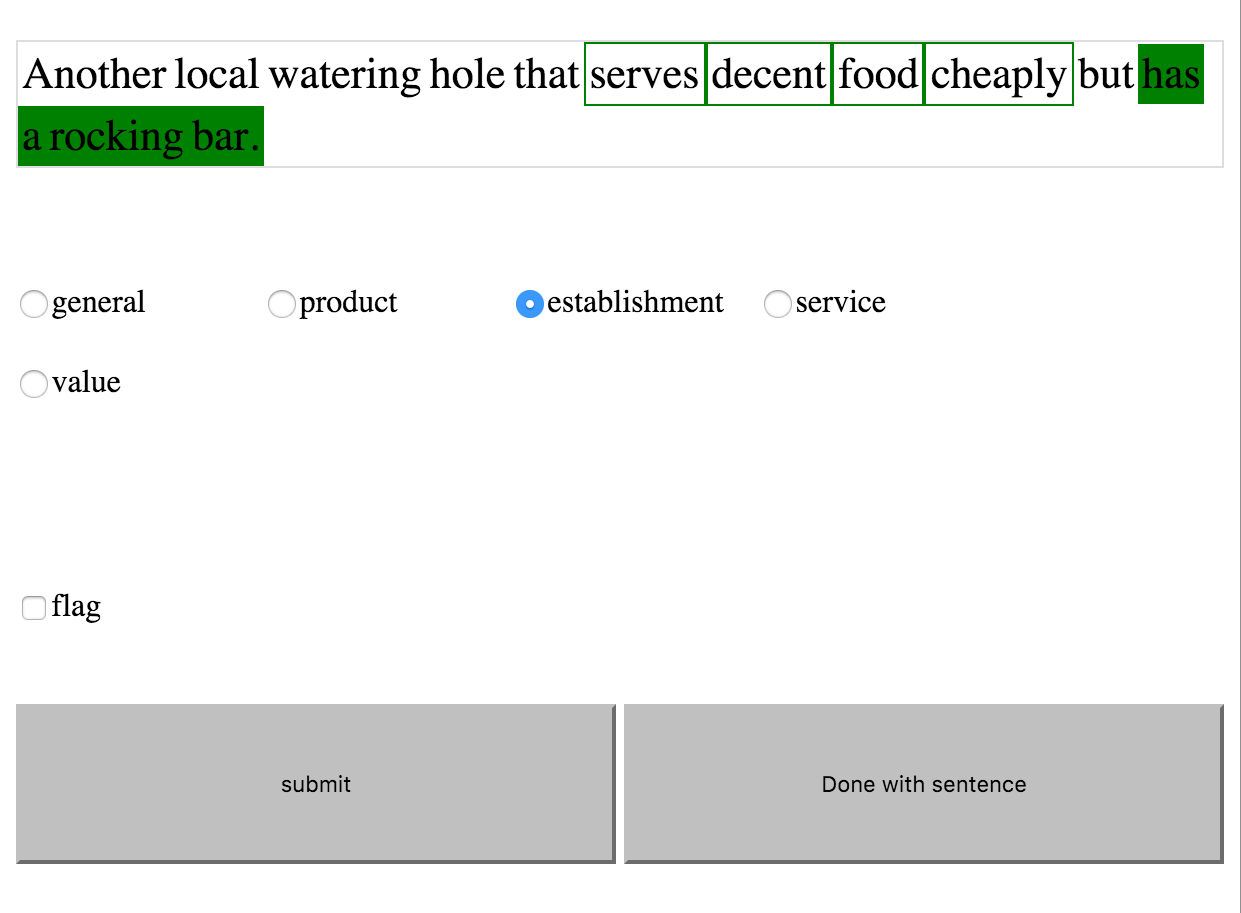
\includegraphics[width=10cm]{annotate_aspect.png}}
  \caption{Aspect level annotation interface. Allows selection of aspects by marking a series of words(dark green). Since a sentence can hold more than one aspect, once an aspect has been submitted, the same sentence is kept and another aspect can be selected(a green border is left to indicate a previous submission).}
  \label{fig:annotate_aspect}
\end{figure}

\begin{figure}[t]
  \centering
  \begin{tikzpicture}

  \begin{axis}[
      %title={Classifier performance per category},
      %xlabel={Categories},
      ylabel={Number of aspects},
      ybar, ymin=0,
      %bar width=20pt,
      xtick=data,
      x tick label style={rotate=45,anchor=east},
      xticklabels from table={data/category_distribution.csv}{category},
      xticklabel style={text height=1.5ex},
      ymajorgrids=true,
      grid style=dashed,
      legend pos=north east,
    ]
    \addplot table [x expr=\coordindex, y=count]{data/category_distribution.csv};
  \end{axis}
  \end{tikzpicture}
  \caption{Number of aspects found for each group when annotating 1,000 sentences.}
  \label{fig:cat_count}
\end{figure}

\subsection{Skewed data}
\label{sec:data_skew}
When dealing with real world data, it is possible that some classes in classification tasks are more
common than others. This has been shown to have consequences both in Bayesian classifiers\cite{rennie2003bias}
and Support Vector Machines\cite{svm_bias}, where both have been shown to favor majority
classes.

%todo 1/n
Not only classification methods, but also precision measures are affected by skewed data. In binary
classification with evenly distributed classes, a classifier that favors one class to the extreme that it
always chooses the same class, still achieves around 0.5 precision since the number of true positives
would equal the proportion of the favored class\footnote{This is in fact be the worst possible result
in the binary case, since any classifier performing consistently worse could be modified to return the
opposite and thus have the inverse precision which would be better.}.
If the evaluation data is also biased towards the same class, that classifier will get even
higher precision, which illustrates how important it is to examine classifier
bias and data distribution.

A simple way to solve problems with disproportionate data is to exclude all but an equal amount
from each class to artificially balance the class distribution,
more commonly referred to as \emph{down-sampling}\cite{provost2000machine}.
This could pose a problem if data is very skewed, as this means that the required
amount of available data effectively is divided by the fraction of the least common class.
However, in this work the data was not skewed enough to motivate studies of more
complicated approaches.

Although down-sampling eliminates bias in evaluations, which makes evaluations between
classifiers more comparable, it also reduces the amount of entries used in evaluations.
Therefore this report will evaluate using unscaled data once classifiers have been
verified to be reasonably unbiased in a per class comparison.


\clearpage
\section{Grouping methodologies}
\subsection{Lexical graph search}
The origins of this method are largely narrated by the introductory section of this chapter;
starting out from bare noun matching and evolving into this algorithm.

Based on the observation that there are usually keywords in a sentence with lexicographical
connection to the desired group, an alternative approach to traditional classification is proposed.
This is motivated since classification models generally need good training data to achieve good results.
The idea for this method is to instead use a lexicon of known word relations to find a path from a query
word to one of few word senses each with predefined group labels, and assign the query word the same label.

Figure~\ref{fig:baklava_lex} shows an example of this premise in action,
where the word relations involved in finding the word ``baklava'' were used,
and that it is closer to \emph{product} than \emph{establishment}.

\begin{table}[b]
  \centering
  \begin{tabular}{| r | l |}
    \hline
    \textbf{Aspect group} & \textbf{Predefined keywords}\\ \hline
    Establishment & \emph{furniture, view, music, loud, appearance, clean, location}\\ \hline
    Product & \emph{food, drink, taste, edible}\\ \hline
    Value & \emph{cheap, price, dollar, buck, lots, bargain}\\ \hline
    Service & \emph{service, quick, attentive, wait}\\ \hline
  \end{tabular}
  \caption{Aspect groups with pre-associated key words. The key words are used as starting points for the graph search in the algorithm, and were chosen by asking three independent people about words they associate with each category, out of which these words were selected by the author.}
  \label{tab:cat_words}
\end{table}

\subsubsection{The algorithm}
Using WordNet's \cite{wordnet} word sense relations, a  breadth first search is conducted
starting at the word senses as predefined in table \ref{tab:cat_words}.

For each word sense, neighboring word senses are acquired, and each time a previously undiscovered word sense
is found, it is assigned to the group of the word sense that led the search to it. In other words, the algorithm
is effectively building a mapping from words to groups, which also allows for quick look-ups later.

This method to categorize individual word senses is then extended to categorize full sentences using
a voting heuristic.

\subsubsection{Voting heuristic}
The heuristic is what classifies sentences into groups.
At its availability is the above mentioned mapping for each word sense in the sentence to a group.
Since word senses can consist of more than one word,
e.g. ``happy hour'', the heuristic iteratively searches for multiple word word-senses,
decreasing in length, starting with the full sentence as one word sense.

Next, a map is built using enabling constant time lookup of not only which group is nearest,
but also the distance $d$ from the word sense to the category.

This is then combined into one score using the following scheme:

\begin{equation} \label{eq:heruistic}
  category(s) =
  \underset{k}{\text{argmax}}
  \sum_{w \in s} categoryScore(w, k)
\end{equation}

\begin{equation} \label{eq:heruistic_d}
  categoryScore(w, k) =
  \begin{cases}
    max(d_*) - d_k(w) + 1, & \text{if}\ k \text{ is the nearest class}\\
    0, & \text{otherwise}
  \end{cases}
\end{equation}

where $d_k(w)$ is the distance from the word sense $w$
to its nearest category and $d_*$ is the highest distance any word in the sentence
has to its nearest category(making the category score for worst scored word in the sentence 1).

This way, for a three word sentence $s=w_1w_2w_3$ with the nearest distances
$d_A(w_1)=4$, $d_A(w_2)=6$ and $d_B(w_3)=3$,
the categories will receive the scores $A=3+1+0$ and $B=0+0+4$, and the highest scoring category $A$
would be selected.

\begin{table}[b]
  \centering
  \begin{tabular}{| l | l |}
    \hline
    \textbf{Included} & \textbf{Excluded} \\ \hline
    getHypernyms() & getTopicMembers() \\
    getHyponyms() & getTopics() \\
    getInstanceHypernyms() & getUsageMembers() \\
    getInstanceHyponyms() & getUsages() \\
    getMemberHolonyms() & \\
    getMemberMeronyms() & \\
    getPartHolonyms() & \\
    getPartMeronyms() & \\
    getRegionMembers() & \\
    getRegions() & \\
    getSubstanceHolonyms() & \\
    getSubstanceMeronyms() & \\
    getSimilar() & \\
    getAttributes() & \\
    getRelated() & \\
    getEntailments() & \\
    getOutcomes() & \\
    getVerbGroup() & \\
    \hline
  \end{tabular}
  \caption{WordNet\cite{wordnet} word sense relation methods: Each method returns a list of word senses with the
    associated relation to the source word sense. Listed by whether or not included in the graph search algorithm.}
  \label{tab:bfs_relation}
\end{table}


\subsubsection{Optimization method}
The method has now been described on an abstract level, but there are still two more things that need to be tweaked for it to work: Which word senses to start the search from, and what relations can be used to find word senses for the next iteration.

It is very important when selecting parameters that the data used for selecting the parameters is different from the data that is used to eventually evaluate the method itself. Parameters can not be tweaked unless new data that previously has not been used for evaluation is available. In this work, the data labeled with aspect groups in section \ref{subsec:getting_data} was randomly sampled into three equal parts: Two parts were continuously reshuffled and divided into training and testing sets, and the third part was only used \emph{exactly once} when the method was decided to be tuned.

The predefined words listed in table \ref{tab:cat_words} were selected by manual trial and error and empirically found to work well in combination. A few more word senses were tried and discarded in this process.

Table \ref{tab:bfs_relation} lists available word relations in WordNet and whether they were included or excluded in the final algorithm. This selection was made in a similar fashion as word senses.

A brief attempt was made to automate selection of these parameters using a hill-climbing algorithm, but this was deemed superfluous and abandoned.

\begin{figure}[t]
  \centering
  \fbox{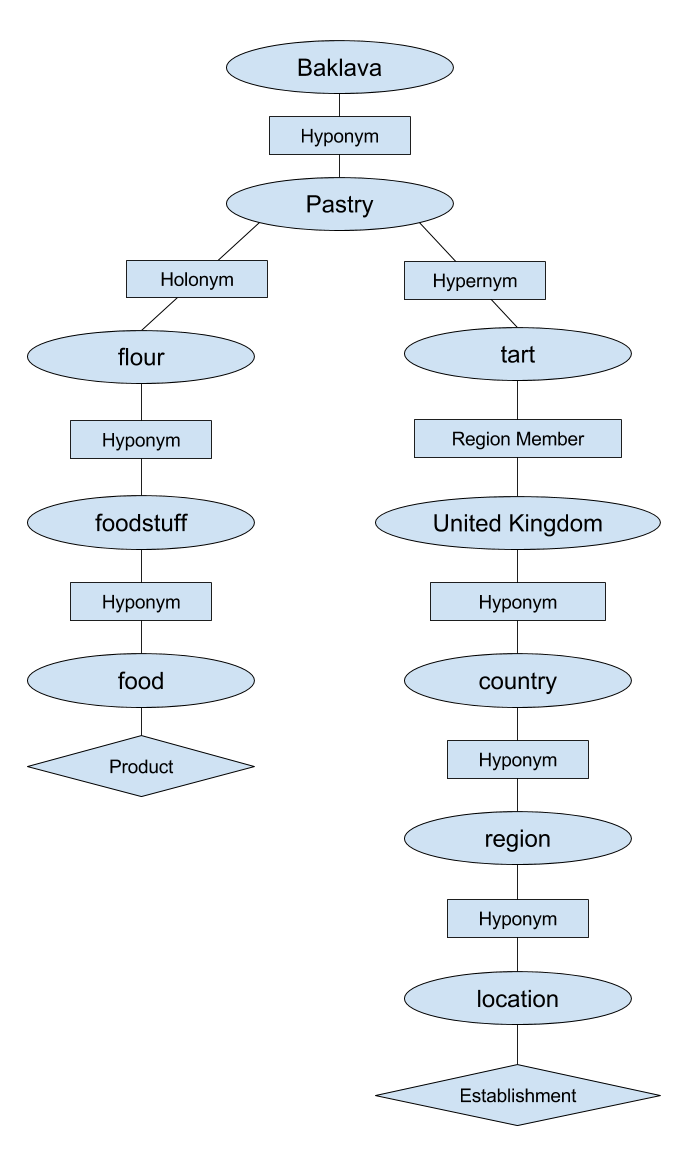
\includegraphics[width=10cm]{img/baklava_lex.png}}
  \caption{Example showing how ``baklava'' could be lexicographically closer to category ``product'' than ``establishment''. Ellipses represent word senses, rectangles the relations between senses, and diamonds predefined categories with a few associated senses (in this case \emph{food} and \emph{location}).}
  \label{fig:baklava_lex}
\end{figure}

\clearpage
\subsection{Machine learning classifiers}
To provide a relatable comparison for the novel algorithm, a series of well known machine learning
classifiers were considered:

Scikit-learn\cite{scikit-learn} is an open source machine learning toolkit which provides various
classifier implementations.
The precision of these classifiers were evaluated individually on my data to decide which classifier to use.

When doing background research for this project, early experiments with ensemble compositions of these classifiers
showed promise, so an ensemble of the top performing classifier for each distinct type of classifier
(Stochastic Gradient Descent, Linear Support Vector, and Multinomial Naive Bayes)
was constructed and evaluated as well. The classifiers were made to work with both unigrams and bigrams
as features (introduced in section \ref{subsec:ngrams}).

Results for these classifiers can be seen in tables
\ref{tab:individual_unigram_accuracy} and \ref{tab:individual_bigram_accuracy}.
Based on these results it was decided to only further study unigram LinearSVC.


\begin{table}[h]
  \centering
  \begin{tabular}{| c | c | c | c | c || c |}
    \hline
    \multicolumn{6}{|c|}{Unigram} \\
    \hline
    \textbf{Model} & Product & Value & Service & Establishment & \emph{Avg.} \\ \hline
    NaiveBayesClassifier& 0.566 & 0.555 & 0.622 & 0.564 & 0.577 \\
    LogisticRegression  & 0.650 & 0.563 & 0.526 & 0.537 & 0.569 \\
    SGDClassifier       & 0.638 & 0.618 & 0.511 & 0.528 & 0.574 \\
    SVC                 & 0.291 & 0.425 & 0.364 & \textbf{0.760} & 0.460 \\
    LinearSVC           & \textbf{0.658} & 0.612 & 0.606 & 0.576 & \textbf{0.613} \\
    MultinomialNB       & 0.657 & \textbf{0.624} & \textbf{0.641} & 0.478 & 0.600 \\
    BernoulliNB         & 0.496 & 0.470 & 0.585 & 0.616 & 0.542 \\
    \hline
    ensemble            & 0.605 & 0.556 & 0.573 & 0.578 & 0.578 \\
    \hline
%    \textbf{Ensamble} & 0.563 \\ %todo OMG
%    \hline
  \end{tabular}
  \caption{Out-of-the-box \textbf{unigram} per class precision of classifiers included in Scikit-learn.
    Best result for each class is highlighted.
  }
  \label{tab:individual_unigram_accuracy}

  \begin{tabular}{| c | c | c | c | c || c |}
    \hline
    \multicolumn{6}{|c|}{Bigram} \\
    \hline
    \textbf{Model} & Product & Value & Service & Establishment & \emph{Avg.} \\ \hline
    NaiveBayesClassifier& 0.149 & 0.229 & \textbf{0.437} & 0.654 & 0.367 \\
    LogisticRegression  & 0.316 & 0.230 & 0.308 & 0.593 & 0.362 \\
    SGDClassifier       & \textbf{0.329} & \textbf{0.350} & 0.406 & 0.357 & 0.361 \\
    SVC                 & 0.203 & 0.154 & 0.278 & 0.670 & 0.326 \\
    LinearSVC           & 0.323 & 0.223 & 0.306 & 0.620 & 0.368 \\
    MultinomialNB       & 0.201 & 0.230 & 0.288 & 0.771 & 0.373 \\
    BernoulliNB         & 0.121 & 0.202 & 0.299 & \textbf{0.802} & 0.356 \\
    \hline
    ensemble            & 0.243 & 0.228 & 0.334 & 0.694 & \textbf{0.375}\\
    \hline
%    \hline
  \end{tabular}
  \caption{Out-of-the-box \textbf{bigram} per class precision of classifiers
    included in Scikit-learn. Best result for each class is highlighted.
  }
  \label{tab:individual_bigram_accuracy}
\end{table}


\clearpage


\section{Results}

\subsection{Graph-search classifier}
The graph search found and categorized a total of 78'844 word senses, and as a reminder,
these words are derived from the 21 predefined words in table \ref{tab:cat_words}.

On testing data, the algorithm was optimized up to 83.0\% precision at full recall,
which resulted in 71.8\% precision at 98.5\% recall on the final evaluation data.

\subsection{Machine learning classifiers}

\begin{figure}[h]
  \centering

  \begin{tikzpicture}
    \begin{axis}[
        %title={Classifier performance based on data size},
        xlabel={Training data-set size},
        ylabel={Accuracy (Fraction of correctly classified)},
        %xmin=0.3, xmax=0.7,
        %ymin=0.25, ymax=0.75,
        %xtick={0,20,40,60,80,100},
        %ytick={0,20,40,60,80,100,120},
        legend pos=north west,
        ymajorgrids=true,
        grid style=dashed,
      ]
      %\addplot table [x=n, y=p]{data/data_size_unigram.csv};
      \addplot table [x=n, y=p]{data/data_size_unigram_balanced.csv};
      \addplot table [x=n, y=p]{data/data_size_bigram.csv};
      \legend{
        %biased unigram,
        unigram,
        bigram
      }
    \end{axis}
  \end{tikzpicture}
  \caption{Sentence classification performance based on training data size. Each data point represents a new
    sampling of data into training and evaluation sets, where the x axis represents how many sentences from the
    training set are made available to the classifier. The full testing sample set was used in each data point and
    each data point had to be classified(recall=1).
  }
  \label{fig:data_size}
\end{figure}


As expected, figure \ref {fig:data_size} shows that increased quantities of training data quickly yield improved results. This increment starts out approximately linear and eventually converges towards constant as the classifier becomes ``saturated'' with training data. %todo

\pagebreak

\subsection{Per class classification}
\label{sec:per_cat}
\begin{figure}[h]
  \centering
  \begin{tikzpicture}

  \begin{axis}[
      %title={Classifier performance per category},
      %xlabel={Categories},
      ylabel={Per class recall},
      ybar, ymin=0,
      %bar width=20pt,
      xtick=data,
      x tick label style={rotate=45,anchor=east},
      xticklabels from table={data/per_category_unigram.csv}{n},
      xticklabel style={text height=1.5ex},
      ymajorgrids=true,
      grid style=dashed,
      legend pos=north east,
    ]
    \addplot table [x expr=\coordindex, y=p]{data/per_category_unigram.csv};
    \addplot table [x expr=\coordindex, y=p]{data/per_category_unigram_unbalanced.csv};
    \addplot table [x expr=\coordindex, y=p]{data/per_category_bigram.csv};
    \addplot table [x expr=\coordindex, y=p]{data/per_category_bigram_unbalanced.csv};
    \legend{Down-sampled unigram, Unmodified unigram, Down-sampled bigram, Unmodified bigram}
  \end{axis}
  \end{tikzpicture}
  \caption{Down-sampled vs. not down-sampled classifier comparison. Each column on the X-axis represents evaluation sentences with that true class, and the Y-axis shows the fraction of those sentences that were correctly classified.
    Each bar should be compared with its corresponding bars in the other columns. As an example, the second leftmost (red) bar in each column can be seen to have more bias towards common classes than the leftmost (blue) bar in each column, which is the down-sampled version of the same classifier. Comparison with figure \ref{fig:cat_count} will confirm that this bias correlates with the distribution of classes in the data set. No confidence threshold was set in this experiment.}
  \label{fig:per_cat}
\end{figure}


Section \ref{sec:data_skew} introduced skewed data and some potential consequences, which motivated more detailed study of classifier results on a per class basis. Figure \ref{fig:per_cat} illustrates how classifiers trained on
down-sampled training data perform notably more consistent between classes, and that the biased classifier has inflated average precision (accuracy) because of this bias.

Comparison between the balanced/unbalanced versions of the classifier models show that, as expected, there seems to be bias towards the more frequent $product$-class and respectively against the infrequent $value$-class.

It can also be seen that the bigram model is performing poorly for all labels except the \emph{product} class, but it should be noted that this is consistent between the balanced and unbalanced version of the model.


\begin{table}[h]
  \centering
  \pgfplotstabletypeset[
    columns={method,p,r},
    col sep=comma,
    every head row/.style={after row=\midrule},
    columns/method/.style={string type,column type=l, column name=Classifier},
    columns/p/.style={precision=3, column type=l, zerofill, column name=Precision},
    columns/r/.style={precision=4, column type=l, column name=Recall},
  ]{data/general_aspect.csv}

  \vspace{0.4cm}\caption{Result summary}
  \label{general_asp}
\end{table}

\section{Discussion}
\subsection{Algorithmic graph search classifier}
As results show, it is possible to categorize aspects using a lexical database.

What is particularly interesting about this result is that, although the method is evaluated in a supervised
manner, the heuristic is in itself unsupervised, and could be used with in a unsupervised manner, although it would impossible to know know how the method is performing without labeled evaluation data.

\subsection{Machine Learning classifiers}

Figure \ref{fig:data_size} surprises me in that bigram features appear ``saturated'' at as little as 500 sentences.
It would have been my expectation that bigrams would eventually achieve better performance than unigrams, but
with a learning curve that increases slower with more training data.

A possible explanation could be that in the classified sentences a only few words are key for the assigned class,
so when bigrams are used and that important word only is evaluated in bigrams with its immediate neighboring words,
the cases where neither of those bigrams are found are hurting results more than the added context from the neighboring words.

For example; in the sentence ``I really like their prices'', the entire word is classified based on the word ``prices'', and replacing that word with something else, like ``soups'' would directly change the outcome for the entire sentence. Even if a bigram classifier has seen a sentence like ``This place has great prices'' when training it would be of no help as there the sentences share no bigrams, whereas the unigram classifier may have picked up that the presence of the word ``prices'' correlates with the value group.

If this is the reason why the bigram classifier is performing poorly, it may be that the classifier will need orders
of magnitude more data before it starts performing.


\subsection{Comparison}
Despite better performance, there are a few reasons why I would caution against using the graph search algorithm:

The main reason is that this work includes no study for this method on a per category basis.
As section \ref{sec:data_skew} describes, results are
susceptible to favor classifiers that are biased towards the more common classes; my suspicion is that
the product category is greatly favoured by the graph search method and that results are therefore inflated.
This notion originates in my anecdotal observations when using the full system.

The machine learning classifier on the other hand, was shown to yield much less biased results
when trained on down-sampled results (section \ref{sec:per_cat}), albeit at the cost of
decrease in average performance.

Something to keep in mind about my results is that with a small data-set,
there is real risk of methods becoming too specific towards the training data.
This is known in statistical modeling as \emph{over fitting},
and the same phenomenon can very well appear when modeling with heuristics.
Based on anecdotal observations using my full system, I think there is reason to believe that
the graph search algorithm is suffering from over fitting.

Another important consideration when choosing between these methods is the time invested in their development.
The machine learning classifiers were introduced to give provide a known baseline to compare the graph algorithm,
so no real time was invested in them, and yet they perform similarly. The graph search algorithm on the other hand
required a bit of tinkering to get to the state where it was eventually evaluated.


\chapter{Sentiment Classification}
\label{sec:sentiment_classification}
Sentiment classification is the task of deciding whether sentiment in a sentence
is positive, negative or neutral\cite{nlp_book}.

Sentiment can be derived in various ways. \emph{``I disliked the taste of my coffee''}
is an example of a sentence with negative subjective sentiment.
Subjective sentiments may per definition not apply to everyone.

Sentiment can also be derived from objective sentences:
\emph{``the toilet seat was broken''} clearly implies negative sentiment
as \emph{broken} is an unquestionably negative property for a toilet seat.
Many sentences may be some combination of subjective and objective;
e.g. \emph{``the portion size was small''} is of objective nature,
but holds a subjective definition of what a small portion size is.
And just as objective sentences can hold sentiment, subjective sentences may not, as
the statement \emph{``I thought the wall was red''} illustrates.

This all goes to show that for sentiment classifications, it is insufficient
to use algorithmic or static methods, like the POS-patterns introduced in previous
chapters.

Instead readers will be introduced to a more dynamic statistical method.

\section{Language modeling}

\subsection{\ngram s}
\label{subsec:ngrams}
\ngram~modeling is a versatile, robust and widely used method of modeling languages. Typically the model consists of, for some $n$, all $n$-length sub-sequences of a longer sequence (i.e. one or many documents). Each unique sub-sequence is then referred to as a \ngram, and \ngram s of length \emph{1,2,3} are referred to as \emph{unigrams, bigrams} and \emph{trigrams}, respectively\cite{ngrams}.

Frequencies, counts and occurrences of \ngram s have been used in language modeling\cite{chen_goodman}, text categorization\cite{ngrams}, \todo

As an example, the word-\emph{bigrams} for the sentence \emph{``Languages are fun''} are:
\begin{quote}
  \vspace*{0.1cm}
  \centering
\emph{``\texttt{<BOS>} Languages''}, \emph{``Languages are''}, \emph{``are fun''}, and \emph{``fun \texttt{<EOS>}''}
\end{quote}
where \emph{\texttt{<BOS>}} and \emph{\texttt{<EOS>}} are a tokens representing the start and end of sentences.

Although \ngram~modeling can be applied to virtually any kind of sequence, this report henceforth will refer to \ngram s of words unless otherwise specified.

\subsection{\ngram~language modeling}
If the probability of a word's occurrence in a sentence $P$ is known (e.g. estimated using a corpus), then the probability of a sentence $s$ can be modeled the following way with \emph{unigrams}:

\begin{equation} \label{eq:unigram_chain_prob}
P(s) \approx P(w_1) P(w_2) \dots P(w_n) =\prod_{w_i \in s}P(w_i)
\end{equation}
Similarly, if modeled with \emph{bigrams}:

\begin{equation} \label{eq:bigram_chain_prob}
P(s) \approx P(w_2 | w_1)P(w_3 | w_2) \dots P(w_n | w_{n-1}) = \prod_{w_i \in s}P(w_i|w_{i-1})
\end{equation}
Where $P(w_b | w_a)$ is some probability estimate of a word being $w_b$, provided that the previous word was $w_a$. (Modeling the probability of a word's occurrence solely on previous element(s) in the sequence is know as \emph{the Markov assumption}.) It should be clear that good \ngram~modeling then is about finding a $P$-function that estimates reality well.

A naive \gls{MLE} of a sentence $s$ could be defined something like this:
\begin{equation} \label{eq:bigram_mle}
P(w_i|w_{i-1}) = \frac{c(w_{i-1}\,w_i)}{\sum_{w} c(w_{i-1}\, w_*)}
\end{equation}

Here the number of occurrences where the word $w_{i-1}$ follows $w_i$
(as given by the count function $c$) are normalized by the number of occurrences where $w_{i-1}$
is followed by any word $w_*$, or in other words; the fraction of this particular bigram
out of all bigrams with the same first word.

%\subsection{Why \ngram~s?}
%There are several early studies using publicly available \emph{sentiment lexicons},
%which are corpora of words with associated sentiment scores.
%Readers may be tempted to use such corpora to for 
%
%Human language is full of




\subsection{Properties of different \ngram~lengths}

The length of \ngram s most definitely impact the behaviour of the model.
To illustrate, consider the sentence ``incredibly cheap owners''.

Although the sentence is clearly negative, a unigram model may assign it positive sentiment,
%todo

\section{Smoothing language models}
A common problem when statistically modeling based on existing data,
is how the model should handle previously unseen entities.
Since human language is virtually infinite, even reasonable sentences are innumerable,
and thus handling unseen data is a requirement for good performance.

As can be seen in equation \ref{eq:bigram_mle}, the \gls{MLE} of entities unseen in
training data would per definition be assigned a zero probability, which in turn makes
the chain model(e.g.~\ref{eq:bigram_chain_prob}) assign a zero probability to the entire
sentence\cite{chen_goodman}.

Smoothing is a means of improving models with limited data samples.
It can mitigate the problem of unseen data,
but also makes for better estimations of rare entities, or even combine multiple models.

The rest of this section will introduce a few smoothing methods in a somewhat simplified way.
Methods that combine multiple \ngram~orders will be described only using bigrams and
unigrams for enhanced readability,
but are all generalizable to higher order \ngram~models as well.
For this and a more comprehensible introduction to smoothing,
readers are recommended \emph{(Chen \& Goodman, 1996)}.

\subsection{Additive smoothing}
One of the most basic smoothing techniques called \emph{additive smoothing},
or \emph{Lidstone Smoothing}, introduces a constant $\alpha$ which ensures
non-zero probabilities\cite{chen_goodman}:
\begin{equation} \label{eq:additive_smoothing}
P_{add}(w_i|w_{i-1}) = \frac{c(w_{i-1}\,w_i)+\alpha}{\sum_{w} \big[c(w_{i-1}\, w_*)+\alpha\big]}
\end{equation}
where $0 < \alpha \leq 1$ is commonly used. The case when $\alpha=1$ is also called \emph{Laplace smoothing}\cite{nlp_book}.


\subsection{Interpolated smoothing}
Although additive smoothing addresses unseen data, there are other models that give more accurate estimations.

\emph{Interpolated smoothing} is S. F. Chen and J. Goodman's way of combining models of various complexities,
in this case multiple \ngram~models with different lengths. In interpolation, the probabilities of each model are summed, usually weighted so higher complexity models are given more influence\cite{chen_goodman}.
Below is an example of what most interpolated smoothing approaches look like for bigrams:
\begin{equation}\label{eq:interpolated_smoothing}
  P_{inter}(w_i|w_{i-1}) =
  \lambda_2 P(w_i|w_{i-1}) + \lambda_1 P(w_i)
\end{equation}

where $\lambda_1, \lambda_2$ are weights dividing influence between models, and $\lambda_1 + \lambda_2 = 1$.

Interpolated smoothing techniques provide a simple means of mitigating
the trade-off between complex models with higher confidence
and simpler models that generalize well.
If a queried bigram does not exist in training data at all,
the first term will effectively equal zero,
and the estimate will be the one of a individual unigram model times a reducing factor.

\subsection{Modified Kneser-Ney smoothing}
One of the most commonly used modern smoothing methods is \emph{interpolated Kneser-Ney smoothing},
or \emph{Modified Kneser-Ney smoothing}\cite{nlp_book}, which incorporates two additional intuitions:

Firstly, a high occurrence of higher \ngram s implies at least as high
lower order occurrence. I.e. if the bigram \emph{``San Francisco''} occurs 25 times,
the unigram \emph{``Francisco''} will occur at least 25 times or more.
If the word \emph{``Francisco''} always is preceded by  \emph{``San''},
the probability of other occurrences will be overestimated unigram model.
In Kneser-Ney smoothing, the lower order model is set to be proportional to the
number of times it occurs with \emph{unique histories} divided by the number of times it
occurs with the history in the current \ngram\cite{chen_goodman}, which  in the previous example
works out to be $\frac{1}{25}$.

Higher order models have lesser total counts in their denominator, which means that common
higher order \ngram s, like \emph{``San Francisco''} in our previous example, are assigned high probabilities.
This leads to the second intuition, which is that even few occurrences will
get high probabilities compared to lower order models, which may lead to over-estimations.
This is addressed by subtracting a small \emph{discounting}-constant $D$ in the numerator,
which makes a difference if the count is small, but becomes insignificant small for high counts.
The \emph{modified} part of Modified Kneser-Key smoothing is using different values for this
$D$ depending on the occurrence count of the \ngram~being estimated\cite{chen_goodman}.


\section{Classification methods}
The previous section introduces language modeling, which is used to give the probability of a sentence.
Classification can without much effort be reduced to language modeling, by training one model per class and
selecting the model assigning the highest probability. This is in fact what many common classifiers do.
(In fact, due to the assumption that \ngram~occurrences are independent, e.g. \ref {eq:bigram_mle}
could be viewed as a Naive Bayes classifier with only one class(prior=1).)

\subsection{Choosing a level of analysis}
\label{subsec:sentence_contradictions}
Less than 2\% of sentences with multiple opinions had both positive and negative sentiments.
Furthermore, out of those sentences, X\% were pruned due to sentiment classification falling under the
confidence threshold.

Thus, sentence level was deemed appropriate for sentiment classification.% TODO.


%\subsection{Scikit-learn and other classification methods}
%Scikit-learn\cite{scikit-learn} is a collection of machine learning implementations in Python, ready to use ``out of the box''.
%
%The following methods were examined in this work:
%
%\begin{table}[h]
%  \centering
%  \begin{tabular}{ r l }
%    \textbf{Module name} & \textbf{Explanation}\\
%    GaussianNB (\texttt{GNB}) & Gaussian distributed prior Naive Bayes classifier.\\
%         %& No smoothing (Gaussian prior).\\
%    MultinomialNB (\texttt{MNB}) & Multinomial distributed prior Naive Bayes classifier. \\
%         %& Additive smoothing.\\
%    BernoulliNB (\texttt{BNB})& Bernoulli distributed prior Naive Bayes classifier.\\
%         %& Additive smoothing.\\
%    LogisticRegression (\texttt{LR}) & \\
%    SGDClassifier (\texttt{SGD}) & \\
%    SVC (\texttt{SVC})& \\
%    LinearSVC (\texttt{LSVC}) & \\
%    NuSVC (\texttt{NSVC})& \\
%  \end{tabular}
%  \caption{todo}
%  \label{tab:scikit_classifiers}
%\end{table}
%
%Section \ref{tab:clf_results} shows the individual classifier performances, and based on these results,
%\todo were selected when developing an ensamble classifier. To classify, the ensamble consulted each of
%the included classifiers individually, and selected the class with the highest probability sum(using
%$p=0.75$ \footnote{Selected using binary search between 0.5 and 1.}
%for classifiers based on other concepts than probabilty, like SVCs and Logistic Regression).

%Confidence was defined as the average 


\newpage
\section{Related work}
%Various approaches to sentiment classification exist, where approaches can generally be categorized as either grammatical\cite{todo} or statistical\cite{todo}. This sections aims to give some insight into what has been previously done in the field.

\subsubsection{Chen, Goodman (1996)}
In the thorough study ``An empirical study of smoothing techniques for language modeling.'' smoothing is
thoroughly studied with regard to language modeling. Furthermore, a novel variation of an existing
smoothing technique is introduced, \emph{Modified Kneser-Ney}-smoothing, which outperforms other
smoothing methods to date.


\subsubsection{Turney (2002)}
In early work, Peter Turney classified sentiment of reviews for \emph{automobiles}, \emph{banks}, \emph{movies} and \emph{travel destinations} with accuracies ranging from 66-84\%, by extracting aspects using predefined POS-patterns, and querying search engines for the co-occurrence between found patterns and the words \emph{``excellent''} and \emph{``poor''}\cite{turney2002thumbs}.

\subsubsection{Hu, Liu (2004)}
In ``Mining Opinion Features in Customer Reviews'', reviews are POS-tagged and common data mining methods are used to on to find patterns that extract features(aspects). Sentiment classification is mentioned, but results are presented in a subsequent paper.

\subsubsection{Hu, Liu (2004)}
In ``Mining and summarizing customer reviews'',
previous work by the same authors is extended
with sentiment classification to produce product summaries.

Sentiment is classified by using words in a \emph{sentiment lexicon},
which is extended by word relations in WordNet. Their method also searches for nearby
\emph{negation words}, which if found,
simply negate the outcome of the classification.

Finally a summary is produced, but this process is very briefly described, and is without evaluations. To my understanding, opinions are solely grouped on the lemmatized form of explicit aspects.


\pagebreak
\section{Experiment setup}

\subsection{Available data}

\subsubsection{Training data: Yelp academic data set}
From the Yelp academic data set\footnote{https://www.yelp.com/dataset\_challenge/},
reviews were randomly selected from 900940 positive reviews (rating the business 5/5)
and 260492 negative reviews(rating the business 1/5).%Most reviews consist of more than one sentence.

Based on an underlying assumption that positive reviews consist predominantly of more
positive than negative language, and vice versa for negative reviews,
sentences were labeled as positive or negative depending on what review they originated from.

These reviews were used to train and \emph{balance} classifiers.

\subsubsection{Evaluation data: Sentiment labeled sentences}
Yelp has a data set with 3216 positive and 1271 negative sentences labeled
according to their sentiment towards the the business in general.
These were used to as final evaluation data for the sentiment classifiers.

\vspace{2cm}
\begin{table}[h]
  \centering
  \begin{tabular}{| c | c |}
    \hline
    \textbf{Model} & \textbf{Found \ngram s}\\ \hline
    Unigram&8772\\
    Bigram&55295\\
    Trigram&92569\\
    \hline
  \end{tabular}
  \caption{Number of unique \ngram s found in the same data set for different \ngram~lengths}
  \label{tab:found_ngrams}
\end{table}

\pagebreak


\subsection{Studied classifiers}
To examine the behavior of \ngram~models and the effects of smoothing,
three \ngram~classifiers (unigram, bigram and trigram) with additive smoothing
were developed, based on the probability definition in equation \ref{eq:additive_smoothing}.

The classifiers were trained on 8'000 sentences from positive and negative reviews.
As features, up to the 30'000 most common \ngram s were used\footnote{As table
\ref{tab:found_ngrams} shows, the unigram model only produces 8772 \ngram s,
in which case all of them were used.}.


Two more classifiers were developed with \emph{interpolated} smoothing as suggested in e.g.
\ref{eq:interpolated_smoothing}, by combining the above mentioned classifiers;
\texttt{interpol2} is the linear combination of the unigram- and bigram classifiers, and \texttt{interpol3}
also included the trigram classifier.

\subsubsection{Choosing $\lambda$}
In my experiments $\lambda_1 = \lambda_2 = 0.5$ yielded the best results; this was concluded after a binary search
on repeatedly re-sampled training and testing data found the optimal to be near as makes no difference $0.5$.

Similarly, for \texttt{interpol3} the procedure was repeated for $\lambda_3$ with $\lambda_1 = \lambda_2$ as an added
constraint, and I found again that $\lambda_1 = \lambda_2 = lambda_3 = \frac{1}{3}$ was close enough to optimal.

Note that these values may be dependent on both the data and data size that is used, but these may be good starting
values as it is convenient to have one less parameter to tune.


\subsubsection{Balancing Classifiers}
\label{subsec:sent_balance}
Section \ref{sec:data_skew} introduces imbalanced classes in data, and in section \ref{sec:per_cat} down-sampling is shown to have direct impact on classifier bias. To reduce bias in sentiment classifiers, each of the base classifiers
were balanced to minimize bias. This was done by interactively retraining the classifier with updated fraction between positive reviews in training data.


\pagebreak
\section{Results}

\begin{figure}[h]
  \centering
  \begin{tikzpicture}
    \begin{axis}[
        xlabel={Recall},
        ylabel={Precision},
        xmin=0.4, xmax=1,
        %ymin=0.4, ymax=1,
        %xtick={0,20,40,60,80,100},
        %ytick={0,20,40,60,80,100,120},
        legend pos=north east,
        ymajorgrids=true,
        grid style=dashed,
      ]
      %\addplot table [x=r, y=p]{data/sent_yelp_pr.csv};
      \addplot table [x=r, y=p]{data/sent_unnorm_unigram_pr.csv};
      \addplot table [x=r, y=p]{data/sent_unnorm_bigram_pr.csv};
      \addplot table [x=r, y=p]{data/sent_unnorm_trigram_pr.csv};
      \addplot table [x=r, y=p]{data/sent_unnorm_interpol_12_pr.csv};
      \addplot table [x=r, y=p]{data/sent_unnorm_interpol_123_pr.csv};
      \legend{
        %yelp..,
        \texttt{Unigram},
        \texttt{Bigram},
        \texttt{Trigram},
        \texttt{Interpol2},
        \texttt{Interpol3},
      }
    \end{axis}
  \end{tikzpicture}
  \caption{Sentiment classifier precision vs. recall. Each dot represents a
    10\% increase in confidence threshold (starting with 1.0 at the left).}
  \label{fig:sent_pr_curve} 
\end{figure}



\subsection{Introducing confidence thresholds}
Figure \ref{fig:sent_pr_curve} shows how the interpolated classifiers have
consistently better performance than the additively smoothed classifiers.
More specifically \texttt{interpol3} also outperforms \texttt{interpol2}, which
not surprisingly supports that adding another model to the interpolation improved results.

The same figure also shows how standalone \ngram~models perform for various values for $n$
(\texttt{unigram}, \texttt{bigram} and \texttt{trigram}).
Precision at full recall directly relates with the order of the model, as lower order
models achieve slightly better performance than higher order models.
However, when confidence thresholds are higher, as recall declines,
higher order models perform better, which can be most clearly seen for the trigram model.

Figure \ref{fig:sent_bias} shows how classifiers have a slight bias towards the positive class.
%, despite the efforts of balancing introduced in section \ref{subsec:sent_balance}.

\newpage

\subsection{Balancing classifiers}
\begin{figure}[h]
  \centering
  \begin{tikzpicture}

  \begin{axis}[
      %title={Classifier performance per category},
      %xlabel={Categories},
      ylabel={Per class recall},
      ybar, ymin=0, ymax=1,
      %bar width=20pt,
      xtick=data,
      x tick label style={rotate=45,anchor=east},
      xticklabels from table={data/sent_pos.csv}{l},
      xticklabel style={text height=1.5ex},
      ymajorgrids=true,
      grid style=dashed,
      legend pos=south west,
    ]
    %\addplot table [x expr=\coordindex, y=p]{data/sent_yelp.csv};
    \addplot table [x expr=\coordindex, y=p]{data/sent_pos.csv};
    \addplot table [x expr=\coordindex, y=p]{data/sent_neg.csv};
    %\addplot table [x expr=\coordindex, y=p]{data/sent_bigram.csv};
    %\addplot table [x expr=\coordindex, y=p]{data/sent_interpol.csv};
    \legend{
      positive, negative
    }
  \end{axis}
  \end{tikzpicture}
  \caption{Performance of classifiers per class. No thresholds(recall=1)}
  \label{fig:sent_bias}
\end{figure}

Figure \ref{fig:sent_bias} shows each classifier's bias after efforts of balancing and table \ref{tab:sent_balances}
shows the distributions that were found optimal.

Notable is the bias the trigram classifier exhibits despite being significantly sampled towards negative reviews.
Further down sampling the positive class had no impact on recall for the \emph{negative}-class, but started to
negatively impact recall for the \emph{positive}-class.


\begin{table}[b]
  \centering
  \begin{tabular}{| c | c | c |}
    \hline
    \textbf{Model} & \textbf{Positive} & \textbf{Negative}\\ \hline
    Unigram&0.47& 0.53\\
    Bigram&0.37&0.63\\
    Trigram&0.26&0.74\\
    \hline
  \end{tabular}
  \caption{Fraction of positive vs negative reviews used when training each base classifier.}
  \label{tab:sent_balances}
\end{table}


\newpage
\section{Discussion}
Of the results shown in Figure \ref{fig:sent_pr_curve}, the most important 
is the effectiveness of smoothing.
Prior to smoothing, I tried various ways of sampling \ngram~s, stemming, lemmatization, stop-lists and entropy estimation of individual \ngram s with little gain. None of the things tried for feature selection resulted in consistent performance gain like did smoothing, where even one of the most basic methods increased overall performance by 5\% units, without any compromises.

The same figure also shows how \ngram~models perform for various values for $n$.
As shown, the performance at full recall directly relates to the order of the
\ngram~model, but that at lower recall the same relationship is inversed. I believe this
to support the hypothesis that lower order \ngram~models generalize better, as opposed to higher order
models which exhibit higher confidence but in fewer entities.


%It should be noted that the comparison between \ysc~and the other models is unfair, since the \ysc~has been trained on more data and has been rigurously tested and reviewed. It is solely included to give perspective on performance of the simpler models.

I do not believe the slight bias seen for the interpolated \ref{fig:sent_bias} affects the outcome of the
system in a noticeable way. I believe one reason why the bias is hard to completely balance is inherent in the data:
positive reviews are generally more expressive of sentiment while negative reviews tend to be more objective and
explanatory. I have also anecdotally heard from other data scientists at Yelp that have had similar observations.

That said, it could arguably be a desired property for real world applications to have slight bias towards the majority class
to have statistical models align better with reality. One may even argue that in this particular case there can be some social benefit to positive bias as well.


\subsection{Further improving results}
I am convinced that exploring smoothing further, and in particular Modified Kneser-Ney,
is a reliable way of further improving sentiment classification results. I did not include the
mathematical representations of this smoothing because open sourced implementations exist
that are probably worthwhile looking into, such as \emph{KenLM}\cite{kenlm}. However, interested readers will not
be disappointed reading \emph{Chen \& Goodman(1996)}\cite{chen_goodman}.


%todo test various feature counts ??

% logical negation might clash with higher order n-gram models
% introducing neutral-class
% actually training to identify positive reviews, not positive statements


\subsection{\ngram~model shortcomings}
\ngram~language models are popular because they are powerful despite their simplicity. They are however not
perfect, and they do have some shortcomings which are worth mentioning.

One is that they rely on semantically high locality in sentences to work. In the English language, meaning of words
may be dependent or affected by other parts of a sentence or even a different sentence altogether.

For example, in the sentence \emph{``If their dishes were cheaper, I'd be the first in line to sing praise how they are redefining healthy eating.''} the beginning of the sentence tells us that what follows is a hypothetical. But because of the words between the beginning and the described hypothetical it would be impossible to incorporate the
true meaning of the benzene into a \ngram~model alone. Higher order \ngram s would not suffice because each added order greatly decreases the probability that the \ngram~ will exist in training data, and \ngram s long enough to cover the start and the end of the sentence will only match that exact sentence and thus won't generalize well.

%todo: cite nlp book


% ``I would've most likely ordered dessert if I had more time and if the waitress was not too busy''
% ``we had the deep fried scallops ($14) nice and juicy.''
% ignored comparative sentiments
% ``The dining room with  low lighting is casual with comfortable booths and tables and a separate lounge area with more seating to watch sports''
% ``The', 'menu', 'offers', 'sandwiches', ',', 'appetizers', ',', 'steaks', ',', 'seafood', ',', 'chicken', ',', 'ribs', ',', 'prime', 'rib', ',', 'pasta', ',', 'salads', ',', 'homemade', 'soups', ',', 'and', 'desserts',
% Good food at reasonable prices
% I like beef with potatoes on the side
% I love steaks, ....
% You would think their exorbitant prices would at least buy some decent customer service.
% other restaurants!!!!!

% food is good ole american


% =========================================================================================================


\chapter{Summary}

\subsection{Aspect extraction}
Using pattern based extraction methodologies;
\begin{itemize}
\item At least one aspect was found in 78.5\% of reviews, with an average of 2.7 aspects per review.

\item it is estimated that between 62.86\% and 86.67\% of all extracted aspects were relevant(depending on definition of relevant; see section \ref{subsec:aspect_eval}),

\item an estimate calculation finds that for a typical business with around 300 reviews,
approximately \numValueAspects~can be expected for the least common aspect group, which should be enough to make conclusions about that group.
\end{itemize}


\subsection{Aspect grouping}
\begin{itemize}
\item Unigram LinearSVC with 61.3\% accuracy, was found the most effective classifier from selection of classifiers in scikit-learn,
\item bigrams are found to perform poorly as features,
\item down-sampling majority classes reduces machine learning classifier's bias towards common classes and
  significantly improves recall for minority classes,
\item and the graph search classifier is found to achieve 71.8\% accuracy, but is suspected to be biased towards
  majority classes, required greater effort to implement and may be over fitted to the small data set that was used.

\end{itemize}


\subsection{Sentiment classification}
In this chapter;

\begin{itemize}
\item Sentiment is accurately classified with 75.1\% accuracy, or 89.1\% at 69.6\% recall,
\item the classifiers are shown to be almost impartial (75.3\% vs 69.1\% per class recall),
\item interpolated smoothing techniques are found to give unconditionally better accuracy than additive smoothing,
\item interpolating three models is found more effective than interpolating two models,
\item and lower order n-gram models are shown to generalize slightly better but have lower confidence than higher order models.
\end{itemize}

\section{Conclusions}

There are three general overall conclusions in this report.

The first one is the effectiveness and versatility \ngram~ language modeling.
A good language model and understanding of it can be used to solve all three
tasks covered in this report, should be considered a worth an investment of time.

Another conclusion is the usefulness of evaluating results on a \emph{per class} basis;
results can be inflated by bias which is hidden unless results are broken down for each class.

Finally, I found it effective to break down the full system into smaller tasks which could be studied in more detail.
Being able to measure success of each task enables further improvement to the system in a measurable way.


\subsection{Obstacles and lessons learned}


\subsubsection{Individual studies of tasks}
The decision to study each task individually helped isolating concerns and understanding system behavior as a whole. But, it took a bit of back-and-fourth to figure out what my exact boundaries of the system should be. Updating one tasks would change its requirements for the other tasks, which meant they needed to be updated as well.

My processes was to first get a very simple prototype running with all the tasks included; and then move on to study each step in isolation in order to improve overall results. I do believe in defining the performance of the full system as the product of its task's performance, but I also found that it is easy to focus too much on individual tasks and forgetting about the system as a whole. I think it would have helped my process to reevaluate the full system between each iteration on a sub-task. After all, each improvement to a sub-task should be done with an improvement of the full system in mind.

\subsubsection{Data annotation}
I ended up re-annotating data several times. The idea of \emph{``I'm gonna get it right the first time, so I don't have to do over''} led me to initially annotate in a too detailed and inconsistent fashion, which in turn made it complicated to extract conclusions. For example, in a sentence like \emph{``The servants were friendly''}, should the entire sentence be annotated as positive for \emph{service}, or just the word \emph{``servants''}? And if the former method is used, how should cases with multiple aspects (\emph{``Both service and food was excellent''}) be handled?

Especially hard was annotating for aspect grouping, as I didn't have a clear idea of what I wanted the outcome to be. Further, I was also inconsistent about whether or not to include classes for \emph{other} and \emph{neutral}, and how to handle sentences that didn't quite fit what I was annotating. I think a general lesson is to annotate exactly for the task you want to solve, and only consider adding complexities in the context of the purpose of the data, as added detail does come with a cost when using the data.

The data annotations interface itself didn't take long to develop and was helpful because clicking on a word is simpler than e.g. typing its position in the sentence, but it did serve as bit of a distraction as anything that wasn't originally supported, had to be tinkered with manually. This was fun, but not productive towards the end goal. A sufficient alternative would have been to simply use a digital spreadsheet.


\subsubsection{The Classifier Store}
Although it is an implementation detail, I think something worth mentioning is the classifier store,
because it worked well and saved time over the course of the project. Through out the code base,
classifiers were not instantiated like regular objects, but instead requested in what I call the
classifier store.
Upon request, the store would inspect the module containing the source code that trains
the requested classifier and make a hash value based on this inspection.
Once the classifier has been trained, a binary dump of that classifier is be made in a file with a name
corresponding to that hash.

This way, the same classifier will automatically be reused until a change is made to 
its source code, which reduces the training time (about 3 minutes) to the time to
read the binary dump (about a second).

This turned out especially useful when composing classifiers out of several other classifiers.


%\subsection{Reinforcement learning}
%Something that hasn't been covered but I find very interesting is the idea of incorporating reinforcement learning for the system as a whole. This could be done by preseting users with the end results and asking them whether they are correct. I believe this could be effective for a few reasons: For starters, I belive it to be more interesting to 

%\subsection{Know your data?}

%\subsection{The General aspect}


%\subsection{Focus on things unique for a place}

\newpage

\section{Final words}
Initially my hope was that this report would cover only one of the three tasks introduced, but in more depth. Because of the project being hosted abroad, I began background studies and preparation on my own and most of these preparations turned out to overlap with already existing solutions at my host company. Although unfortunate, it was still a great learning experience; after studying a problem on my own, I got to compare the solutions I had come up with with existing production systems and got professional feedback on my own experiments.

In search for a less explored task, I read up on aspect extraction and grouping as well, and also got to familiarize myself with the workings of existing solutions to these problems at Yelp, with the goal of being able to reuse and possibly improve one of these existing systems.

I got these systems to running in isolation and produced results that I could compare with my own, however, halfway through my internship, I decided to abandon this path for two reasons: Most importantly, I was running out of time. These systems were designed to run on Yelp's infrastructure, which I would lose access to as my internship finished. Secondly, because these were production systems, they were built to work reliably at much larger scale. So they had additional additional mechanisms for monitoring, graceful error handling, and working in a distributed context, which is all out of scope for this work and would have slowed down my experiments.

Instead, I decided to focus on putting my learnings about the overarching problem from this project in writing, along with some experiments designed to illustrate these findings. The result is what you are now reading. It is my hope that this document could prove as an introduction and help someone unacquainted focus on the right things, and even though the results are humble,
the introduced setup is well suited for further work to improve these results.



\bibliographystyle{plain}
\bibliography{references}

\end{document}
 
